\section{Introduction}
\label{sec:intro}

\begin{figure*}[t]
    \centering
    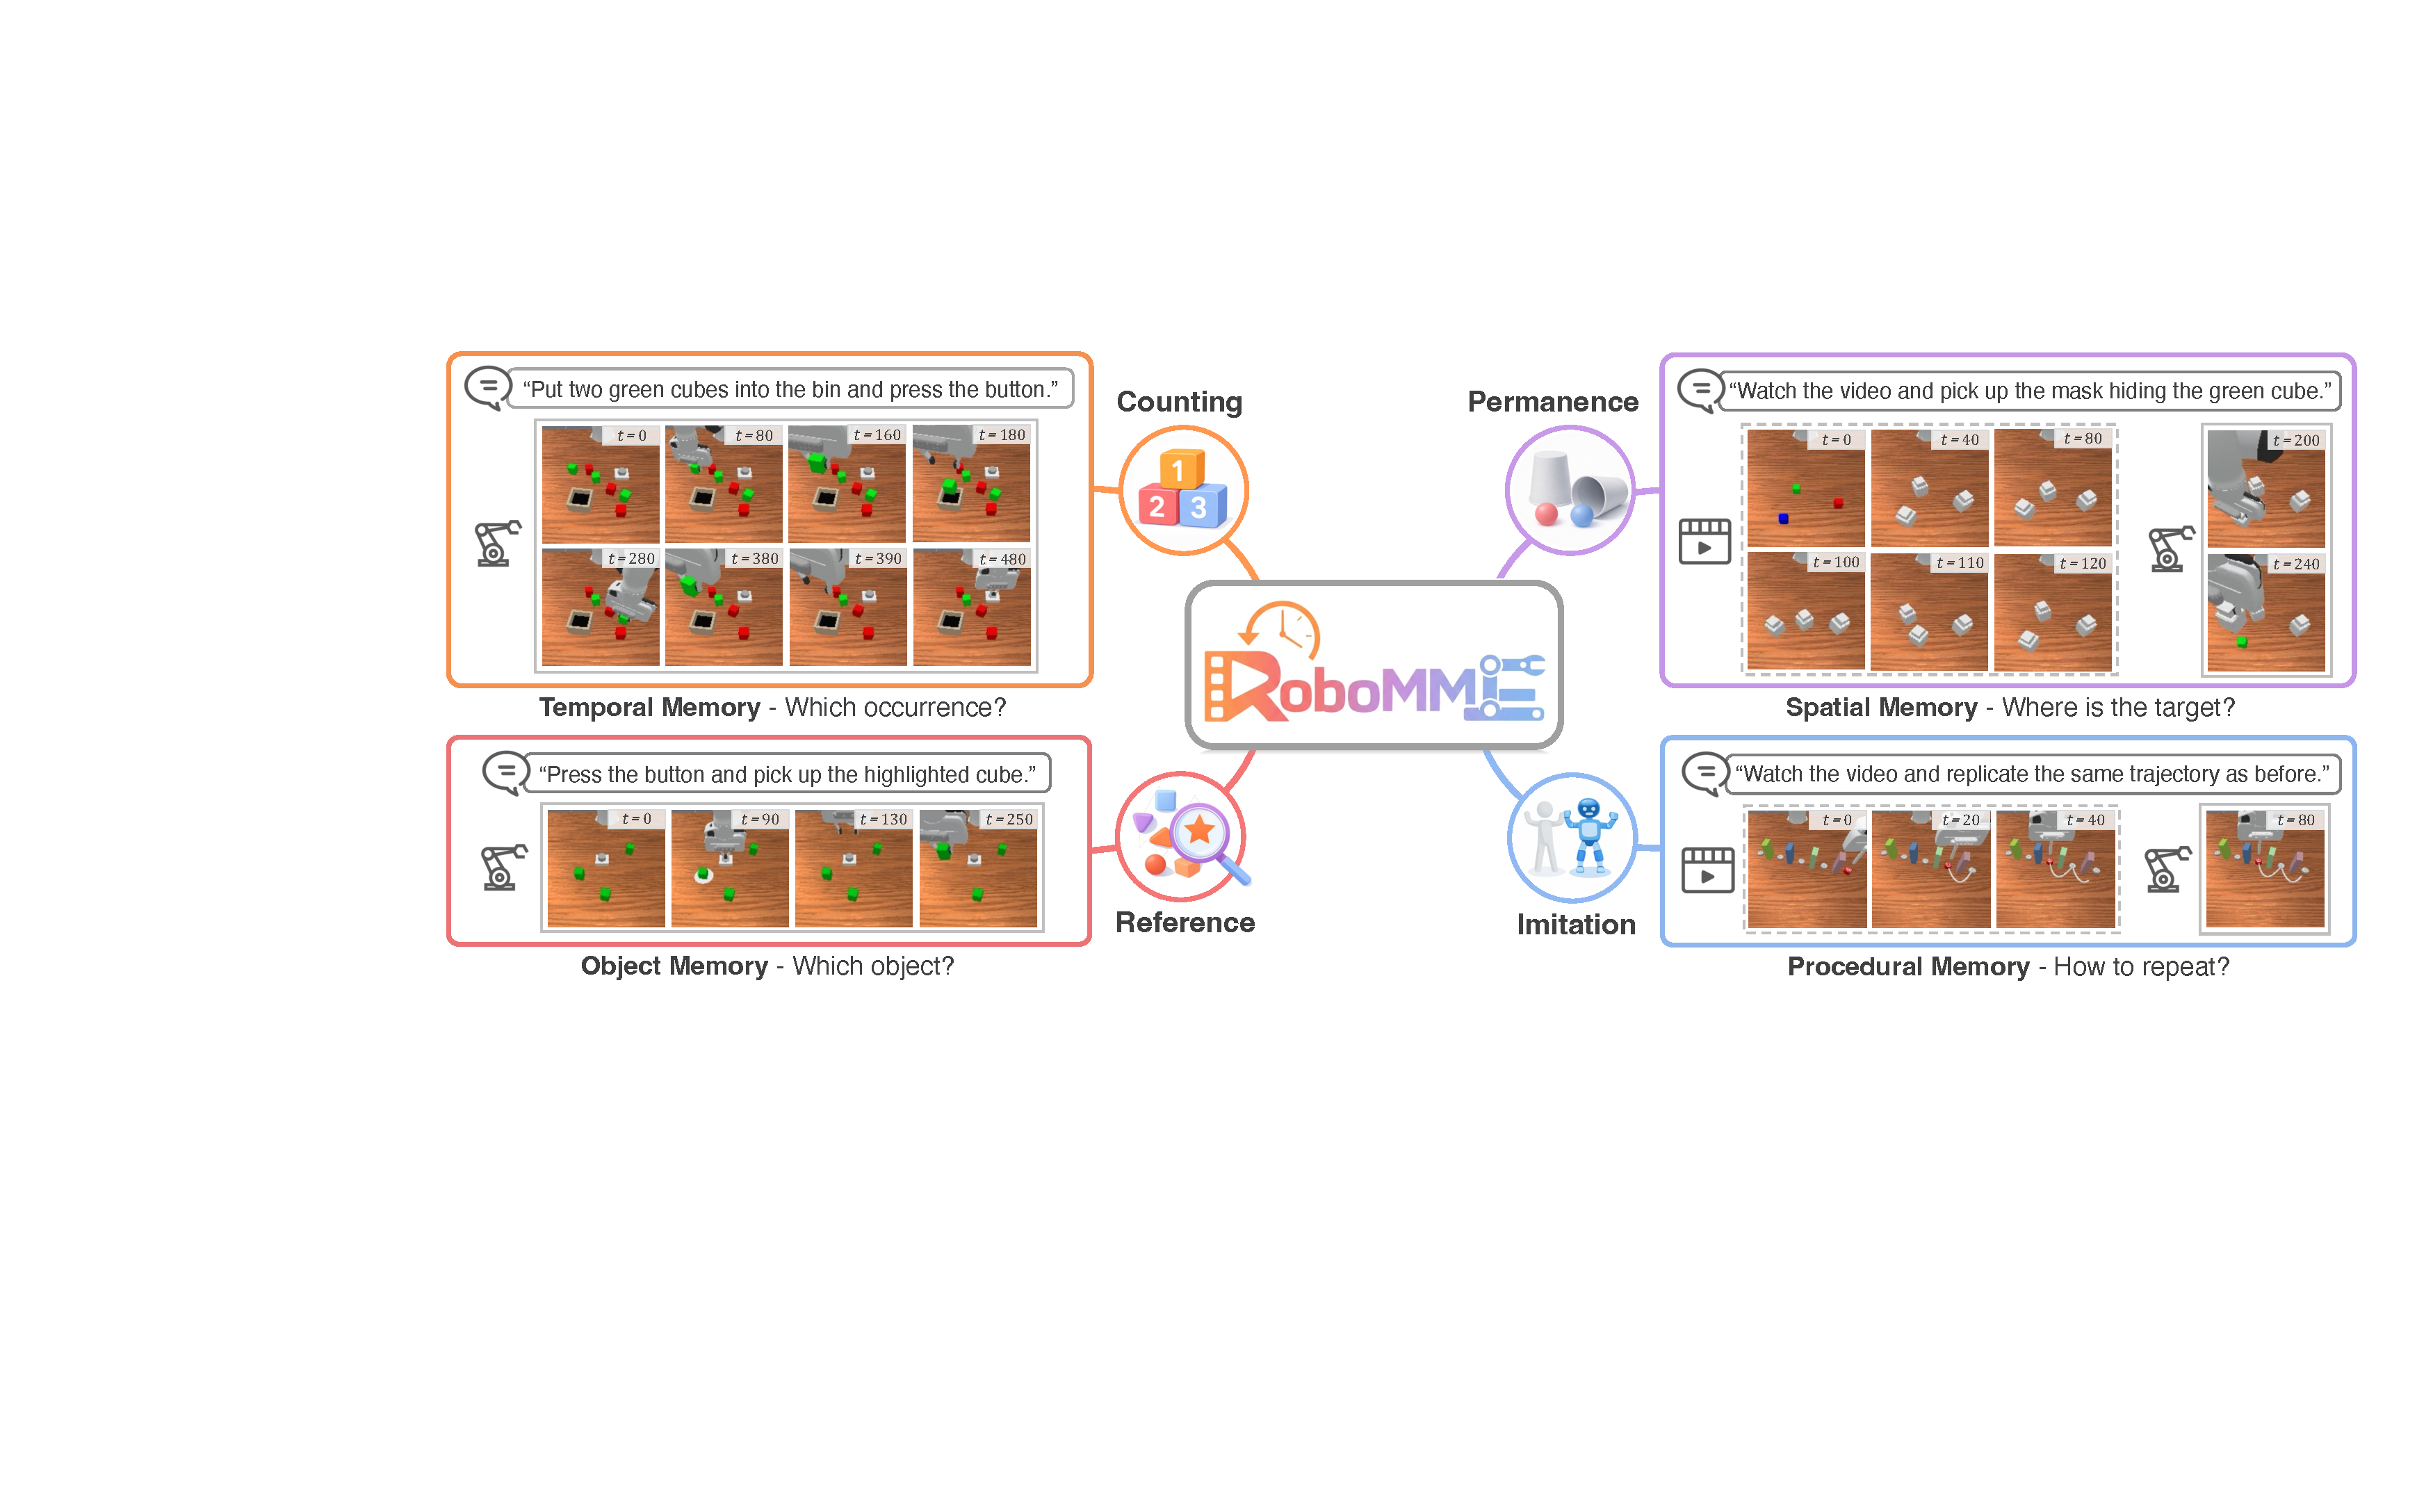
\includegraphics[width=\textwidth]{images/robomme_bench.pdf}
    \caption{\textbf{\benchname}\xspace is a large-scale robotic benchmark for evaluating memory-augmented manipulation, comprising four task suites that emphasize distinct memory demands.
    (1) The \TSone\xspace suite targets \textit{temporal memory}, requiring robots to accumulate and reason over past events, e.g., counting placed green cubes and stopping correctly (top-left).
    (2) The \TStwo\xspace suite focuses on \textit{spatial memory}, requiring tracking of object locations under occlusion and environmental changes, e.g., resolving the correct mask after green and blue cubes swap positions (top-right).
    (3) The \TSthree\xspace suite evaluates \textit{object memory}, requiring identification under varied referential cues, e.g., recalling a briefly highlighted cube during a button press (bottom-left).
    (4) The \TSfour\xspace suite assesses \textit{procedural memory}, measuring the ability to reproduce previously demonstrated behaviors, e.g., replicating a demonstrated trajectory (bottom-right).
    Overall, \benchname\xspace includes 16 tasks with \trainsteps\xspace high-quality training timesteps for systematic evaluation of memory-augmented policies.}
    \label{fig:teaser}
\end{figure*}

Open-world robotic manipulation often requires reasoning over history and recalling information from past interactions.
For instance, a household robot may be asked to return books to their original positions on a shelf, wipe a table for a specified number of cleaning passes, or fold laundry after observing a human demonstration.
In such scenarios, relying solely on immediate perception for action prediction is insufficient. Effective execution depends on the ability to retain and reuse relevant information across time, which we broadly refer to as \textit{memory}.

Prior work incorporates memory into robotic manipulation policies through three main representations:
(1) \textit{symbolic memory}, which summarizes history using non-differentiable abstractions, such as point-tracking trajectories \cite{chen2025history} and language-based subgoals \cite{sridhar2025memer};
(2) \textit{perceptual memory}, which represents history as a group of visual features, including  multi-frame visual tokens \cite{jang2025contextvla} and memory banks \cite{fang2025sam2act, shi2025memoryvla};
and (3) \textit{recurrent memory}, which compresses contextual features into fixed-size latent states through recurrent models \cite{zhou2025mtil, liu2024robomamba}.
While demonstrating the importance of memory, these methods rely on different policy backbones and inconsistent evaluation protocols, making it unclear which memory designs generalize across tasks.
Progress is further limited by the absence of benchmarks that capture diverse and challenging memory requirements.
Existing benchmarks either address limited memory types or lack sufficient demonstrations, preventing systematic evaluation.

To address these limitations, we present \textbf{\benchname}: a unified large-scale \underline{\textbf{Robo}}tic simulation benchmark designed for \underline{\textbf{M}}emory-augmented \underline{\textbf{M}}anipulation \underline{\textbf{E}}valuation.
Drawing inspiration from cognitive theories of human memory \cite{atkinson1968human}, \benchname\xspace categorizes memory into four cognitive dimensions: (1) \textit{temporal memory} for event accumulation and ordering; (2) \textit{spatial memory} for tracking object locations under occlusion and scene change; (3) \textit{object memory} for resolving referential identity across time; and (4) \textit{procedural memory} for reproducing previously demonstrated motion patterns. These memory types define four corresponding task suites, \TSone, \TStwo, \TSthree, and \TSfour, respectively, each composed of four carefully designed tasks. In total, \benchname\xspace contains 16 diverse long-horizon tasks with 1,600 demonstrations, yielding \trainsteps\xspace high-quality timesteps for comprehensive evaluation of memory-augmented policies.

Building on \benchname, we develop a family of 14 memory-augmented VLA models based on the $\pi_{0.5}$ backbone \cite{pi05} to systematically study how different memory representations influence manipulation performance.
Neural representations are integrated through three strategies---memory-as-context, memory-as-modulator, and memory-as-expert---as detailed in \cref{sec:method}.

Interestingly, our experiments show that no single memory representation or integration strategy consistently performs well across all tasks, indicating that conclusions from prior work may not generalize. Instead, effectiveness is highly task-dependent: symbolic memory excels at counting and short-horizon reasoning, while perceptual memory is critical for time-sensitive and motion-centric behaviors. Among all variants, perceptual memory combined with the memory-as-modulator design achieves the best balance between performance and computational efficiency. Together, these results establish the first comprehensive framework for understanding memory in manipulation, and represent a step toward reliable, long-horizon, history-dependent robotic generalist policies.
